\documentclass{article}
\usepackage[margin=1in]{geometry}
\usepackage{tikz}
\usepackage{pgfplots}
\pgfplotsset{compat=1.18}
\usetikzlibrary{arrows.meta, positioning, calc, shapes.geometric, decorations.fractals}

\title{LaTeX Image Creation Showcase}
\author{Generated by ChatGPT}
\date{\today}

\begin{document}
\maketitle
\tableofcontents

\newpage

\section{Overlapping Colour Circles}
This simple diagram relies solely on the \texttt{tikz} package.
\subsection*{Packages}
\begin{itemize}
    \item \texttt{tikz}
\end{itemize}
\subsection*{Steps}
\begin{enumerate}
    \item Start a \texttt{tikzpicture} environment.
    \item Fill three unit circles with different colours at offset positions.
    \item The overlaps naturally blend the colours.
\end{enumerate}
\begin{figure}[h!]
    \centering
    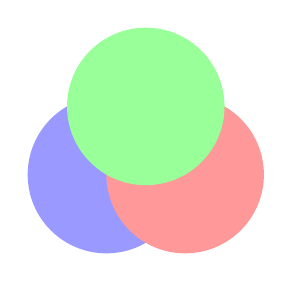
\begin{tikzpicture}
        \fill[blue!40] (0,0) circle (1);
        \fill[red!40] (1,0) circle (1);
        \fill[green!40] (0.5,0.866) circle (1);
    \end{tikzpicture}
    \caption{Overlapping primary colour circles}
\end{figure}

\newpage

\section{Sine and Cosine Curves}
This plot uses \texttt{pgfplots} on top of TikZ to create axis-aligned graphs.
\subsection*{Packages}
\begin{itemize}
    \item \texttt{tikz}
    \item \texttt{pgfplots}
\end{itemize}
\subsection*{Steps}
\begin{enumerate}
    \item Begin a \texttt{tikzpicture} and then an \texttt{axis} environment.
    \item Plot the sine function with a solid blue line.
    \item Plot the cosine function with a red dashed line.
\end{enumerate}
\begin{figure}[h!]
    \centering
    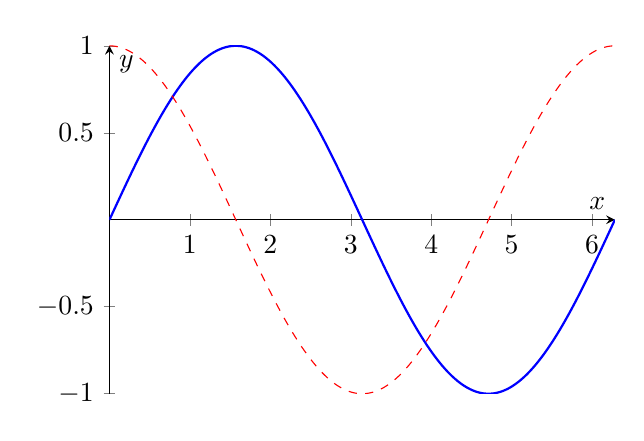
\begin{tikzpicture}
        \begin{axis}[width=8cm,height=6cm,axis lines=middle,samples=200,domain=0:6.283,xlabel=$x$,ylabel=$y$]
            \addplot[blue,thick] {sin(deg(x))};
            \addplot[red,dashed] {cos(deg(x))};
        \end{axis}
    \end{tikzpicture}
    \caption{Sine and cosine curves}
\end{figure}

\newpage

\section{3D Gaussian Surface}
The surface is produced with \texttt{pgfplots}' three--dimensional plotting capabilities.
\subsection*{Packages}
\begin{itemize}
    \item \texttt{tikz}
    \item \texttt{pgfplots}
\end{itemize}
\subsection*{Steps}
\begin{enumerate}
    \item Open a \texttt{tikzpicture} and an \texttt{axis} with a 3D view.
    \item Use \texttt{addplot3} with a Gaussian function over a grid.
    \item Apply a colour map for visual depth.
\end{enumerate}
\begin{figure}[h!]
    \centering
    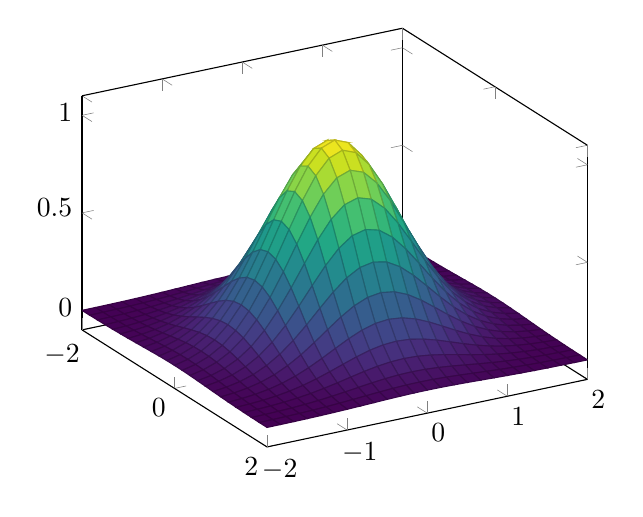
\begin{tikzpicture}
        \begin{axis}[view={60}{30},colormap/viridis,width=8cm]
            \addplot3[surf,domain=-2:2,domain y=-2:2,samples=25]{exp(-(x^2+y^2))};
        \end{axis}
    \end{tikzpicture}
    \caption{Gaussian surface}
\end{figure}

\newpage

\section{Simple Flowchart}
This diagram uses TikZ's shapes and arrows libraries.
\subsection*{Packages}
\begin{itemize}
    \item \texttt{tikz}
    \item \texttt{arrows.meta}, \texttt{positioning}, \texttt{shapes.geometric}
\end{itemize}
\subsection*{Steps}
\begin{enumerate}
    \item Define styles for process and decision nodes.
    \item Place nodes with relative positioning.
    \item Connect nodes using arrowed paths.
\end{enumerate}
\begin{figure}[h!]
    \centering
    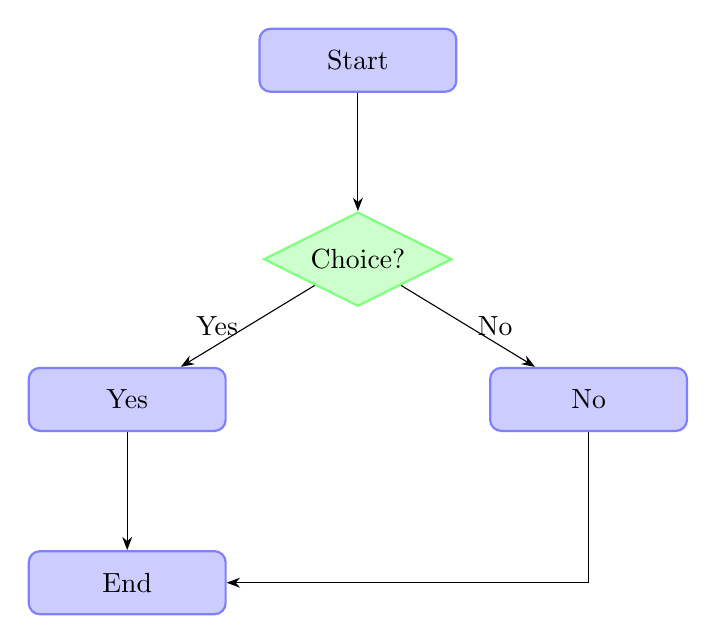
\begin{tikzpicture}[node distance=1.5cm,>=Stealth]
        \tikzstyle{proc}=[rectangle,rounded corners,draw=blue!50,fill=blue!20,thick,minimum width=2.5cm,minimum height=0.8cm]
        \tikzstyle{decision}=[diamond,aspect=2,draw=green!50,fill=green!20,thick,text centered]
        \node[proc] (start) {Start};
        \node[decision,below=of start] (decide) {Choice?};
        \node[proc,below left=of decide] (yes) {Yes};
        \node[proc,below right=of decide] (no) {No};
        \node[proc,below=of yes] (end) {End};
        \draw[->] (start)--(decide);
        \draw[->] (decide)-- node[left]{Yes} (yes);
        \draw[->] (decide)-- node[right]{No} (no);
        \draw[->] (yes)--(end);
        \draw[->] (no)|-(end);
    \end{tikzpicture}
    \caption{Simple flowchart}
\end{figure}

\newpage

\section{Koch Snowflake Fractal}
This fractal uses the \texttt{decorations.fractals} library within TikZ.
\subsection*{Packages}
\begin{itemize}
    \item \texttt{tikz}
    \item \texttt{decorations.fractals}
\end{itemize}
\subsection*{Steps}
\begin{enumerate}
    \item Scale the \texttt{tikzpicture} for visibility.
    \item Draw an equilateral triangle path.
    \item Apply the \texttt{Koch snowflake} decoration to the path.
\end{enumerate}
\begin{figure}[h!]
    \centering
    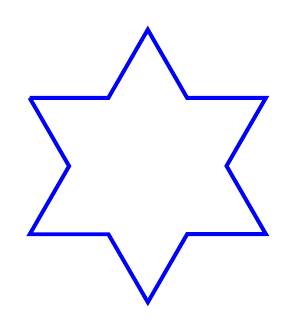
\begin{tikzpicture}[scale=3]
        \draw[blue,line width=0.5mm]
            decorate [decoration=Koch snowflake]
                { -- ++(0:1) -- ++(-120:1) -- ++(-240:1) -- cycle};
    \end{tikzpicture}
    \caption{Koch snowflake fractal}
\end{figure}

\end{document}
